\section{Технологическая часть}

В данном разделе обосновывается выбор средств реализации, приводится описание структуры разработанного программного обеспечения, а также представлены листинги реализации ключевых алгоритмов визуализации и расчета кинематики.

\subsection{Выбор средств реализации}

Для разработки программы был выбран язык программирования C++~\cite{cpp_ref} (стандарт C++20). В качестве графической библиотеки и фреймворка для создания пользовательского интерфейса использована библиотека Qt~\cite{qt_doc} (версия 6). Она предоставляет:
\begin{itemize}
	\item кроссплатформенные средства создания оконного интерфейса (модуль \texttt{QtWidgets});
	\item оптимизированные математические классы (\texttt{QVector3D}, \texttt{QMatrix4x4});
	\item класс \texttt{QImage} для удобного вывода сформированного буфера кадра на экран.
\end{itemize}

Среда разработки --- Zed editor, система сборки --- qmake.

\subsection{Структура программного обеспечения}

Программа реализована с использованием принципов объектно-ориен-тированного программирования. Архитектура приложения включает следующие основные классы и структуры:

\begin{itemize}
	\item \texttt{MainWindow} — класс главного окна приложения. Отвечает за инициализацию графического интерфейса пользователя и обработку сигналов от элементов управления (кнопок, слайдеров, чекбоксов).

	\item \texttt{RenderWidget} — класс виджета для вывода трехмерной графики. Реализует цикл с использованием таймера, обрабатывает события ввода (нажатия клавиш мыши, перемещение курсора, прокрутку колеса) и управляет взаимодействием между пользователем и сценой.

	\item \texttt{Renderer} — класс, инкапсулирующий логику программного рендеринга. Содержит методы для:
	      \begin{itemize}
		      \item трансформации вершин из локального пространства в экранное;
		      \item растеризации треугольников с использованием барицентрических координат;
		      \item управления Z-буфером для удаления невидимых поверхностей;
		      \item расчета освещения по модели Фонга для каждого пикселя;
		      \item отрисовки теней методом планарной проекции.
	      \end{itemize}

	\item \texttt{Scene} — класс, описывающий состояние виртуального мира. Хранит контейнер объектов (шестеренок), параметры гексагональной сетки и геометрию статического окружения (пола). Реализует алгоритмы кинематики: поиск ведущей шестерни, распространение вращения по графу сцеплений и детектирование заклинивания механизма.

	\item \texttt{Camera} — класс виртуальной камеры. Отвечает за формирование матриц вида и проекции. Реализует управление положением наблюдателя в сферических координатах (азимут, угол места, радиус) и предоставляет функционал для генерации лучей из экранных координат в мировое пространство.

	\item \texttt{Gear} — класс, описывающий отдельную шестеренку. Содержит параметры объекта (радиус, количество зубьев, текущий угол поворота) и методы для процедурной генерации полигональной сетки (вершин и нормалей) тела шестерни и её оси вращения.

	\item \texttt{Geom.h} — заголовочный файл, содержащий вспомогательные структуры данных: \texttt{Vertex} (вершина с координатами и нормалью) и \texttt{Triangle} (набор из трех вершин и цвета).
\end{itemize}

\clearpage

Диаграмма классов представлена на рис. \ref{fig:diagram}.

\begin{figure}[H]
	\centering
	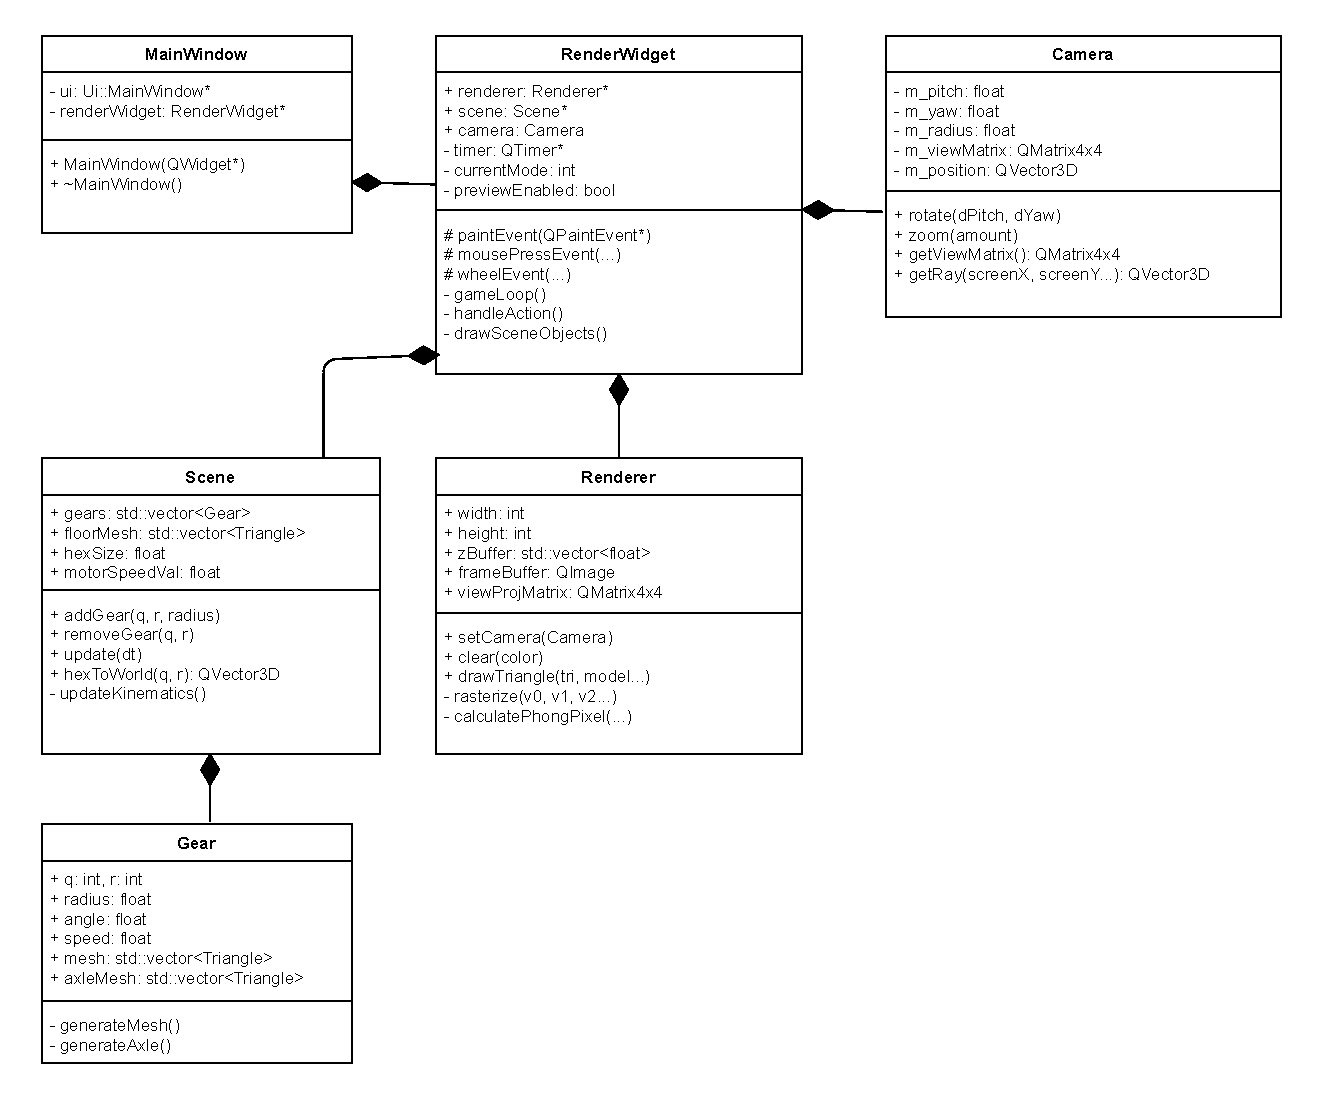
\includegraphics[width=\textwidth]{img/uml.pdf}
	\caption{Диаграмма классов}
	\label{fig:diagram}
\end{figure}

Диаграмма компонентов представлена на рис. \ref{fig:diagram_mod}.

\begin{figure}[H]
	\centering
	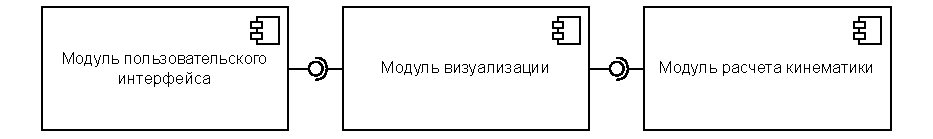
\includegraphics[width=\textwidth]{img/mod.pdf}
	\caption{Диаграмма компонентов}
	\label{fig:diagram_mod}
\end{figure}

\clearpage

\subsection{Реализация алгоритмов визуализации}

Ключевым этапом визуализации является растеризация треугольников с использованием Z-буфера и интерполяцией нормалей для освещения Фонга.

В листинге \ref{lst:rasterize} приведен метод растеризации, который принимает три вершины, прошедшие вершинные преобразования, и заполняет пиксели в буфере кадра.

\begin{lstlisting}[caption={Реализация алгоритма растеризации с Z-буфером}, label={lst:rasterize}]
void Renderer::rasterize(const RasterVertex& v0, const RasterVertex& v1, const RasterVertex& v2, const RenderSettings& settings) {
    int minX = std::max(0, (int)std::min({v0.screenPos.x(), v1.screenPos.x(), ...}));
    int maxX = std::min(width - 1, (int)std::max({v0.screenPos.x(), ...}) + 1);
    int minY = std::max(0, ...}));
    int maxY = std::min(height - 1, ...}) + 1);
    float area = edgeFunction(v0, v1, v2);
    float invArea = 1.0f / area;
    for (int y = minY; y <= maxY; y++) {
        uint32_t* scanline = (uint32_t*)frameBuffer.scanLine(y);
        for (int x = minX; x <= maxX; x++) {
            float w0 = edgeFunction(v1, v2, x, y) * invArea;
            float w1 = edgeFunction(v2, v0, x, y) * invArea;
            float w2 = 1.0f - w0 - w1;
            if (w0 >= 0 && w1 >= 0 && w2 >= 0) {
                float z = w0 * v0.screenPos.z() + w1 * v1.screenPos.z() + ...;
                if (zBufferTest(x, y, z)) {
                    updateZBuffer(x, y, z);
                    if (settings.isShadow) {
                        scanline[x] = qRgb(30, 30, 30);
                    } else {
                        QVector3D normal = v0.normal * w0 + v1.normal * w1 + ...;
                        QVector3D worldPos = v0.worldPos * w0 + v1.worldPos * w1 + ...;
                        scanline[x] = calculatePhongPixel(worldPos, normal, settings);
                    }
                }
            }
        }
    }
}
\end{lstlisting}

\subsection{Реализация алгоритма кинематики}

Для расчета вращения используется алгоритм обхода графа в ширину (BFS). Метод \texttt{updateKinematics} обновляет скорости и углы поворота всех шестеренок в цепи, исходя из параметров ведущей шестерни. Реализация представлена в листинге \ref{lst:kinematics}.

\begin{lstlisting}[caption={Реализация алгоритма расчета кинематики}, label={lst:kinematics}]
void Scene::updateKinematics() {
    for (auto& g : gears) {
        if (!g.isDriver) g.speed = 0;
        else g.speed = driverSpeed;
        g.isJam = false;
    }
    std::queue<int> q;
    q.push(driverIdx);
    visited[driverIdx] = true;

    while(!q.empty()) {
        int currIdx = q.front(); q.pop();
        Gear& curr = gears[currIdx];
        if (curr.isJam) continue;
        for (size_t i = 0; i < gears.size(); i++) {
            if (isConnected(curr, gears[i])) {
                float ratio = curr.radius / gears[i].radius;
                float newSpeed = -curr.speed * ratio;
                if (visited[i]) {
                    if (std::abs(gears[i].speed - newSpeed) > EPSILON) {
                        curr.isJam = true;
                    }
                } else {
                    gears[i].speed = newSpeed;
                    visited[i] = true;
                    syncPhase(curr, gears[i]);
                    q.push((int)i);
                }
            }
        }
    }
}
\end{lstlisting}

\subsection{Интерфейс пользователя}

Графический интерфейс пользователя (GUI) разработан с использованием дизайнера форм Qt Designer и сохранен в файле \texttt{MainWindow.ui}. Интерфейс включает в себя:
\begin{enumerate}
	\item Область рендеринга: занимает большую часть окна, отображает трехмерную сцену. Поддерживает управление камерой мышью (ЛКМ — вращение, колесо — масштабирование).
	\item Панель управления: расположена слева и содержит:
	      \begin{itemize}
		      \item выбор размера добавляемой шестерни;
		      \item режим удаления объектов;
		      \item переключатель режима предпросмотра;
		      \item управление ведущей шестерней: направление (по/против часовой) и слайдер скорости.
	      \end{itemize}
\end{enumerate}

Обработка событий ввода реализована в классе \texttt{RenderWidget}. Метод \texttt{handleAction} использует класс \texttt{Camera} для построения луча из точки клика мыши и нахождения соответствующей ячейки гексагональной сетки.

Интерфейс главного окна изображен на рисунке \ref{img:main_window}.

\begin{figure}[H]
	\centering
	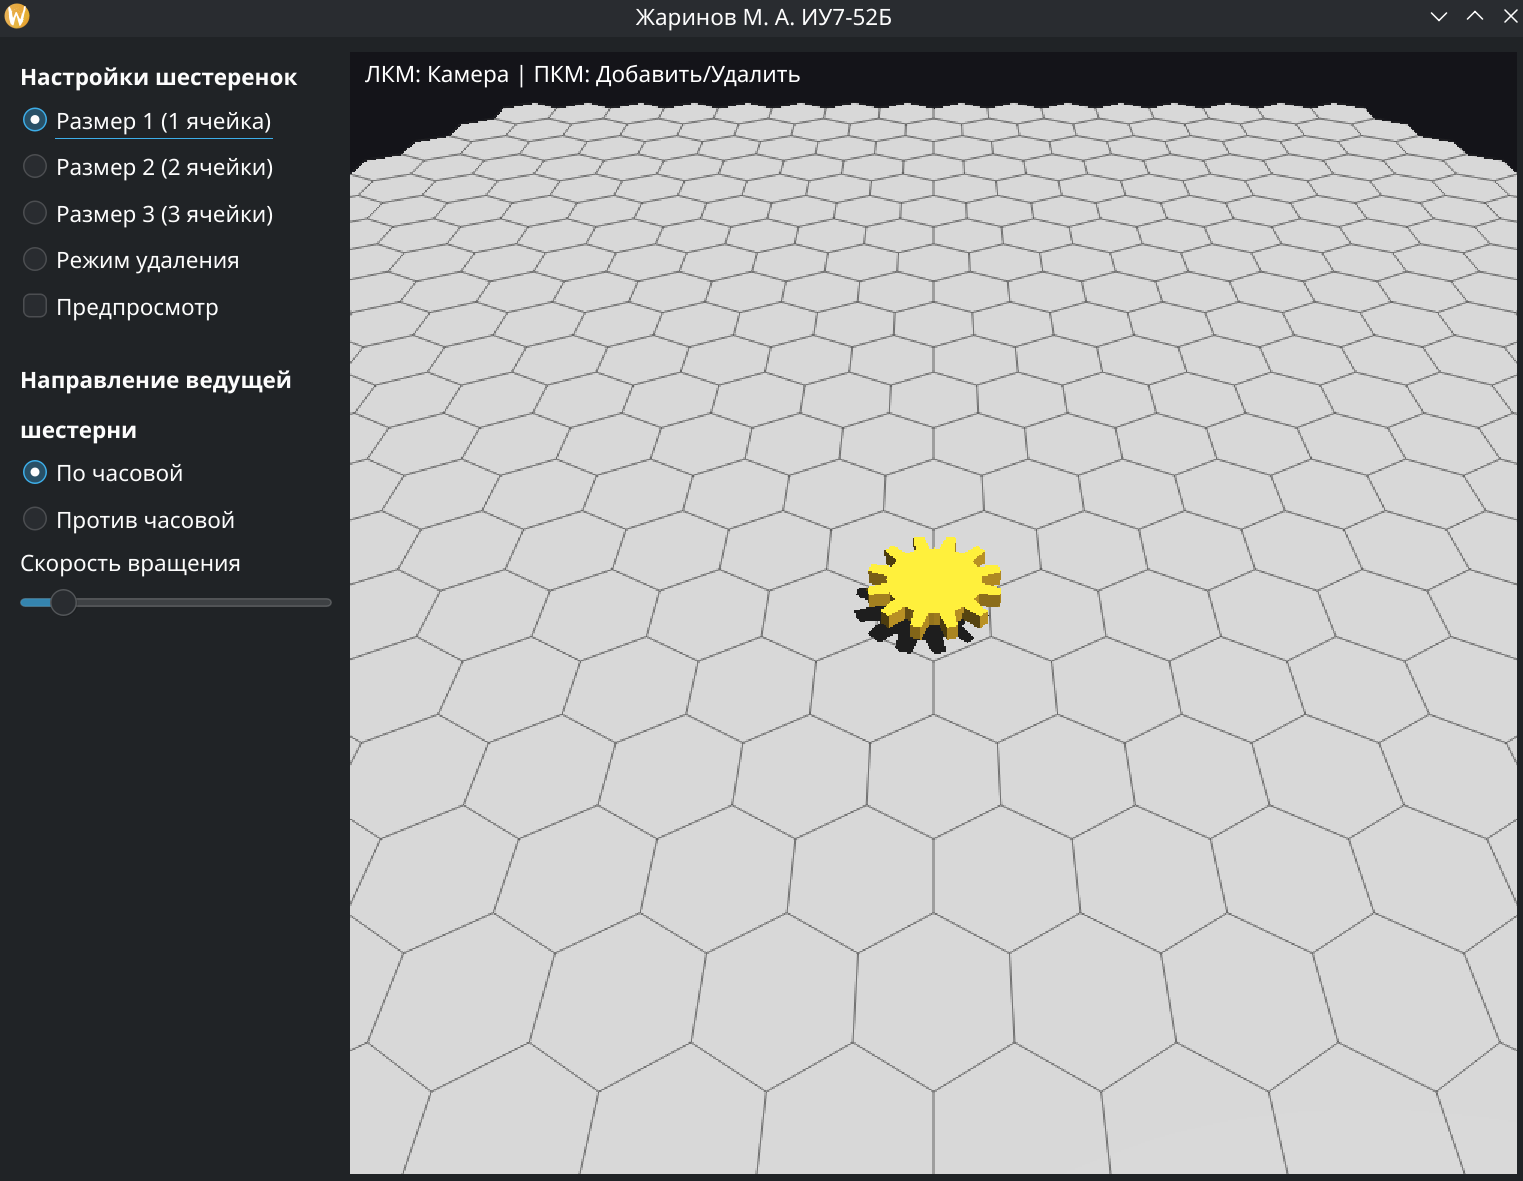
\includegraphics[width=\textwidth]{img/main_window.png}
	\caption{Главное окно программы}
	\label{img:main_window}
\end{figure}

\subsection*{Вывод}

В данном разделе описаны средства реализации и архитектура программного комплекса. Приведены реализации основных алгоритмов: растеризации треугольника с учетом Z-буфера и освещения, а также распространения кинематических связей в системе шестеренок.
